\setcounter{secnumdepth}{4}
\subsection{Multi-task Learning for Chest X-ray Abnormality}
In this paper, researchers built a model trained on 297,541 chest X-rays. The system is based on a novel multi-task deep learning architecture that in addition to classifying and showing a heat-map of the abnormalities also supports the segmentation of the lungs and heart \cite{guendel2019multi}. The research demonstrated that by training the model concurrently on these tasks, one can increase the classification performance. This research produced state of the art performance of 0.883 AUC on average across 12 different abnormalities. ChestX-Ray 14 \cite{wang2017chestx} and PLCO datasets were combined to increase the amount of variability of images and this also showed increase in performance. 

As mentioned before techniques were applied to increase accuracy. One of the methods employed was to normalise the images. A challenge in processing chest radiographs is that there can be large variabilities in the appearance of the image and this is due to the acquisition source, radiation dose \cite{guendel2019multi}. The paper proposes to dynamically window each image by adjusting the brightness and contrast via a linear transformation of the image intensities. Example of output is shown in figure~\ref{fig:Normalisation} 


\begin{figure}[H]
	\centering
	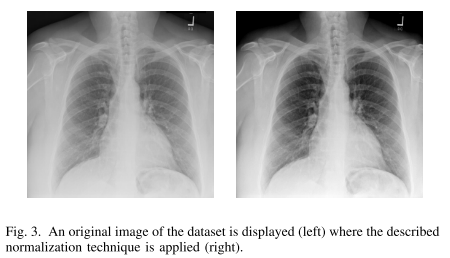
\includegraphics[scale=0.7]{NormalisationTechnique.png}
	\caption{We can see that certain parts of the X-ray become more visible hence making abnormalities more clear for the model}
	\label{fig:Normalisation}
\end{figure}

In addition , the paper also harnesses spatial knowledge related to individual pathologies as well as underlying structure i.e the heart and lungs which can be exploited to increase classification performance. The paper proposes that once can focus the learning task to the heart and lung region as information outside of these regions may be regarded as irrelevant for the diagnosis of heart/lung abnormalities. 

In order to achieve this segmentation, a DenseNet model shown in figure~\ref{fig:DenseNet} \cite{huang2017densely} has been used and figure~\ref{fig:Segmentation}  presents the architecture as well as an example showing the segmentation technique. Another technique that was used to take advantage of spatial information was the use of several approximate spatial labels provided in the PLCO dataset. For five abnormalities(Nodule,Mass,Infiltrate,Atelectasis,Hilar Abnormality) there are rough location information available  to help the model locate where the abnormality is usually located.



\begin{figure}[H]
	\centering
	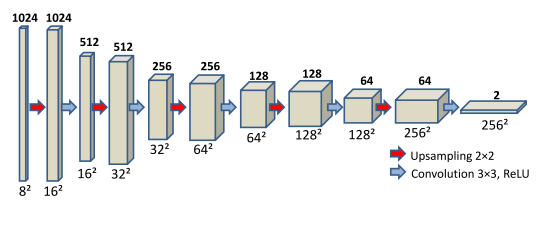
\includegraphics[scale=0.7]{DenseNet_Architecture.png}
	\caption{Architecture for DenseNet}
	\label{fig:DenseNet}
\end{figure}

\begin{figure}[H]
	\centering
	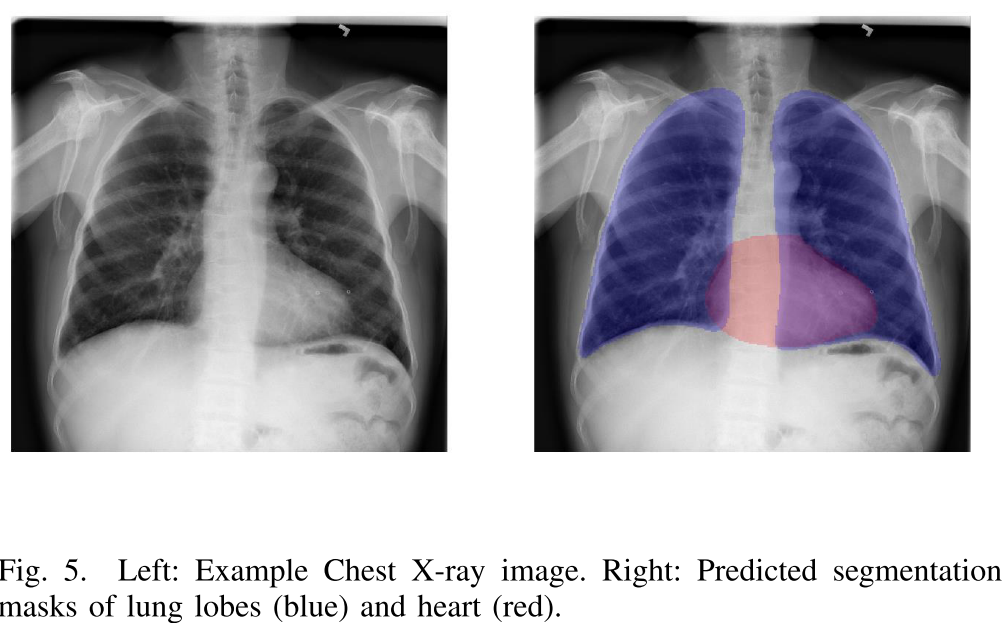
\includegraphics[scale=0.4]{Segmentation.png}
	\caption{Distinct segmentation of lungs and heart}
	\label{fig:Segmentation}
\end{figure}



\subsubsection{Results}


For this paper, different experiments were undertaken to show the performance of the model. As a baseline, performance was measured by only training the classification part on the PLCO dataset. The test was evaluated with an average \textbf{AUC} score across 12 abnormalities of \textbf{0.859}. \par
Results also showed improved classification scores when the network was additionally trained to generate lung and heart segmentation masks (as shown in  figure~\ref{fig:AUC}). Performance increased to 0.866 on average across the abnormalities. \par
As mentioned another technique was to use spatial knowledge and the impact of this showed an average improvement of 0.011\par
This paper also used 2 datasets and by combining both, the average AUC score reaches 0.870. This increase in score is due to more variability in the learning process. As well as this the normalisation technique previously shown in figure~\ref{fig:Normalisation} was applied when training the model and this had a 2 fold benefit. The first was that the training process was reduced on average 2-3 times. The researchers hypothesised that this is due to the images being more aligned in terms of brightness and contrast. Another reason was due to the generalisation of the model parameters and this lead to a performance gain of 0.876. \par
Finally, the researchers upscaled the input image size to 512 in each dimension and adjusted the DenseNet layer to take in 16x16 patch size at each layer. This final network architecture change also added all of the previous techniques mentioned before. The following image shows the results obtained across all techniques and finally the result of combining all the techniques which produces a state-of-the-art performance of \textbf{0.883}



\begin{figure}[H]
	\centering
	\includegraphics[scale=0.4]{AUC_Scores.png}
	\caption{Results showing increasing mean AUC score}
	\label{fig:AUC}
\end{figure}